\section{Future Work}

Several potential directions remain open for further investigation to
deepen and/or improve the study of energy and power monitoring on
AMD processors:

\begin{itemize}
  \item \textbf{Broader hardware coverage:} Evaluate a wider range of AMD
        \gls{CPU} families, including server-grade EPYC generations
        (e.g., Rome, Milan, Genoa), to assess scaling properties and reliability across diverse environments \parencite{hackenberg2019epyc}.
  \item \textbf{Cross-tool comparison:} Systematically compare vendor-provided
        tools such as \textit{e-SMI} \parencite{amd2022esmi}, community
        drivers like \textit{Zenpower}, and \gls{RAPL}-based methods to
        clarify trade-offs in accuracy, portability, and overhead.
  \item \textbf{Sampling-rate exploration:} Investigate further the topic
        higher of higher polling rates of Ryzen’s \gls{SMU} counters, in order
        to establish whether it is possible to enable finer energy
        approximations.
  \item \textbf{Cross-platform studies:} Examine the feasibility of similar
        low-level energy monitoring on non-Linux operating systems, such as
        Windows, to evaluate portability of measurement techniques.
\end{itemize}

An additional research topic could the identification and mapping of the
\gls{CPU} Power Domains in AMD-native solutions for power/energy monitoring. 

\subsection{Methodology Improvements}

The methodology used for this study can be improved/refined in various ways,
as author sees it.

\begin{figure}[h]
    \centering
    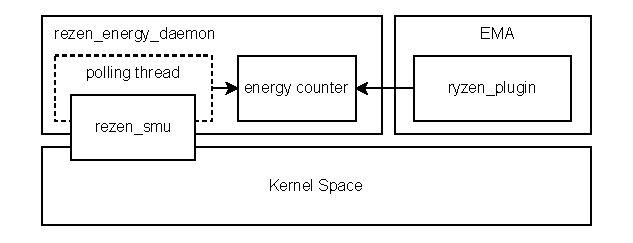
\includegraphics[width=0.7\textwidth]{assets/methodology_improved_concept}
    \caption{
      Suggested improved concept of the \gls{EMA} Ryzen Plugin realization.
    }
    \label{fig:method}
\end{figure}

First, to address the accuracy issues related to Ryzen Plugin readings in
\gls{EMA} a draft concept was developed (see \cref{fig:method}). A dedicated
system daemon process is the core part of this concept. It should be
responsible for polling the power readings via the kernel driver, integrate
them to energy values and update the shared counter, which in turn can be
accessed from user-space in the same fashion as various files in
\texttt{powercap} Linux framework for \gls{RAPL} \footcite{\url{
  https://www.kernel.org/doc/html/latest/power/powercap/powercap.html
}}.

Realization of such method would benefit from higher refresh rates of energy
readings from \gls{PM} Table, thus potentially provide higher accuracy and
precision \cref{sec:find:rates}.

The integration method should also be a target of refinements and
improvements \cref{para:practical}.

The second direction would be revising the realization of \emph{Ryzen Plugin}
for \gls{EMA}, trying to identify any potential bugs, especially related
to numeric type conversions, and precision loss. Topic of counter overflow/
wraparound handling should also be addressed.
